\subsection{Unet architectures}
\label{sec:unets}

The Unet architecture was introduced in \citeA{unet}, explicitly targeting the task of semantic segmentation in biomedical images.
The idea behind this approach is to build upon a fully convolutional network \cite{long2015fully} that extends the CNN models commonly seen for classification.
In particular, the proposed architecture comprises a usual contracting branch supplemented with successive layers where upsampling operators replace pooling counterparts (\cref{fig:unet_architecture}).

The first network portion is built upon a classical block, hereafter referred to as \textit{unet block} or \textit{units}. 
The former is made of two convolutional layers using a varying number of $3\times3$ filters without padding \cite[Section 9.1]{Goodfellow2016deeplearning}, each followed by a \textit{rectified linear unit} (\textit{ReLU}) activation function (\citeNP{fukushima1982neocognitron_relu1, nair2010relu} and \citeNP[Section 6.1]{Goodfellow2016deeplearning}).
This generates an equivalent number of feature maps (or channels) of approximately the same shape as the input image. %depending on the number of filters adopted in each block.
After the previous processing, the resulting feature maps undergo a $2\times2$ max-pooling operation  (\citeNP{weng1993maxpool} and \citeNP[Section 9.3]{Goodfellow2016deeplearning}) with stride 2, thus downsampling the input size.
In practice, the contracting branch takes a grayscale image as input and applies four consecutive unet blocks.
In the first step, 64 filters are adopted, and the downsampling path then continues roughly halving the input size at each block, meanwhile doubling the number of feature channels.
The resulting output consists of 1024 feature maps having approximately $1/16$ the size of the original image.
Finally, the contracting branch ends with the so-called \textit{bottleneck} layer, whereby two \textbox{convolution-activation} blocks are applied.
% which is further processed by a slightly different block (\textit{bottleneck}) whereby two \textbox{convolution-activation} blocks are applied.

Conversely, an almost symmetrical upsampling structure follows in the second part of the network, from which the \textit{U-shape} comes. This time the unet blocks are similar to the ones of the contracting branch except that max-pooling operations are replaced by $2\times2$ up-convolutions \cite{dumoulin2016guideconvolution, zeiler2010deconvolutional} and long-range concatenations.
In this way, the up-convolutions enlarge individual images to nearly double their size. At the same time, the feature channels are halved at each step by the upsampling layer. 
Although this part is crucial to returning an output of a similar shape as the input, the upsampling generally produces blurred pixels that hamper precise localization.
For this reason, each up-convolution is concatenated with \textit{long-range connections}, i.e. the feature channels are integrated by copying a crop of compatible size from the corresponding downsampling block.
As a result, this escamotage establishes a flow of information between lower and higher layers such that both low-level finer details and high-level semantic features contribute to the learning process.
In practice, a total of three upsampling unet blocks are applied in the expanding path, and the architecture terminates with an additional convolutional block.
Specifically, the latter comprises two of the previous \textbox{convolution-activation} blocks followed by a last $1\times1$ convolutional layer to map the resulting 64-component feature vector to the desired number of classes. 
In the case of cell segmentation, this corresponds to two feature maps which can be interpreted as pixel-level scores for the classification as 0 (background) or 1 (signal) classes.

In summary, the Unet architecture aims to create an encoding branch intended to capture relevant features that enable the recognition of the objects without caring where they are placed. Once this goal is achieved, the decoding structure is then applied to refine the localization of the detected objects.

This work considers two implementations of the above structure. The first one corresponds to the original version of \citeA{unet} except for the padding strategy -- we use padded convolution to retain the initial size.
The resulting model will be referred to as \textit{Unet} in the following.
The second, instead, consists of a lighter version obtained by setting the initial number of filters equal to 16 and scaling the following units consequently.
Importantly, three unet blocks are used (plus the bottleneck) rather than the four of the original implementation.
Both of the previous choices are motivated by the intent of testing a unet-like implementation with a comparable number of parameters with respect to the ResUnet alternatives (see \cref{sec:resunets} for more details).
However, a trivial transposition of the original unet blocks does not work in practice for our use case, so we resort to the insertion of additional batch normalization \cite[Section 8.7.1]{Goodfellow2016deeplearning} layers after each \textbox{convolution-activation} block.
The resulting ``light" unet architecture will be referred to as \textit{small Unet} hereafter.

\begin{figure}
\centerline{
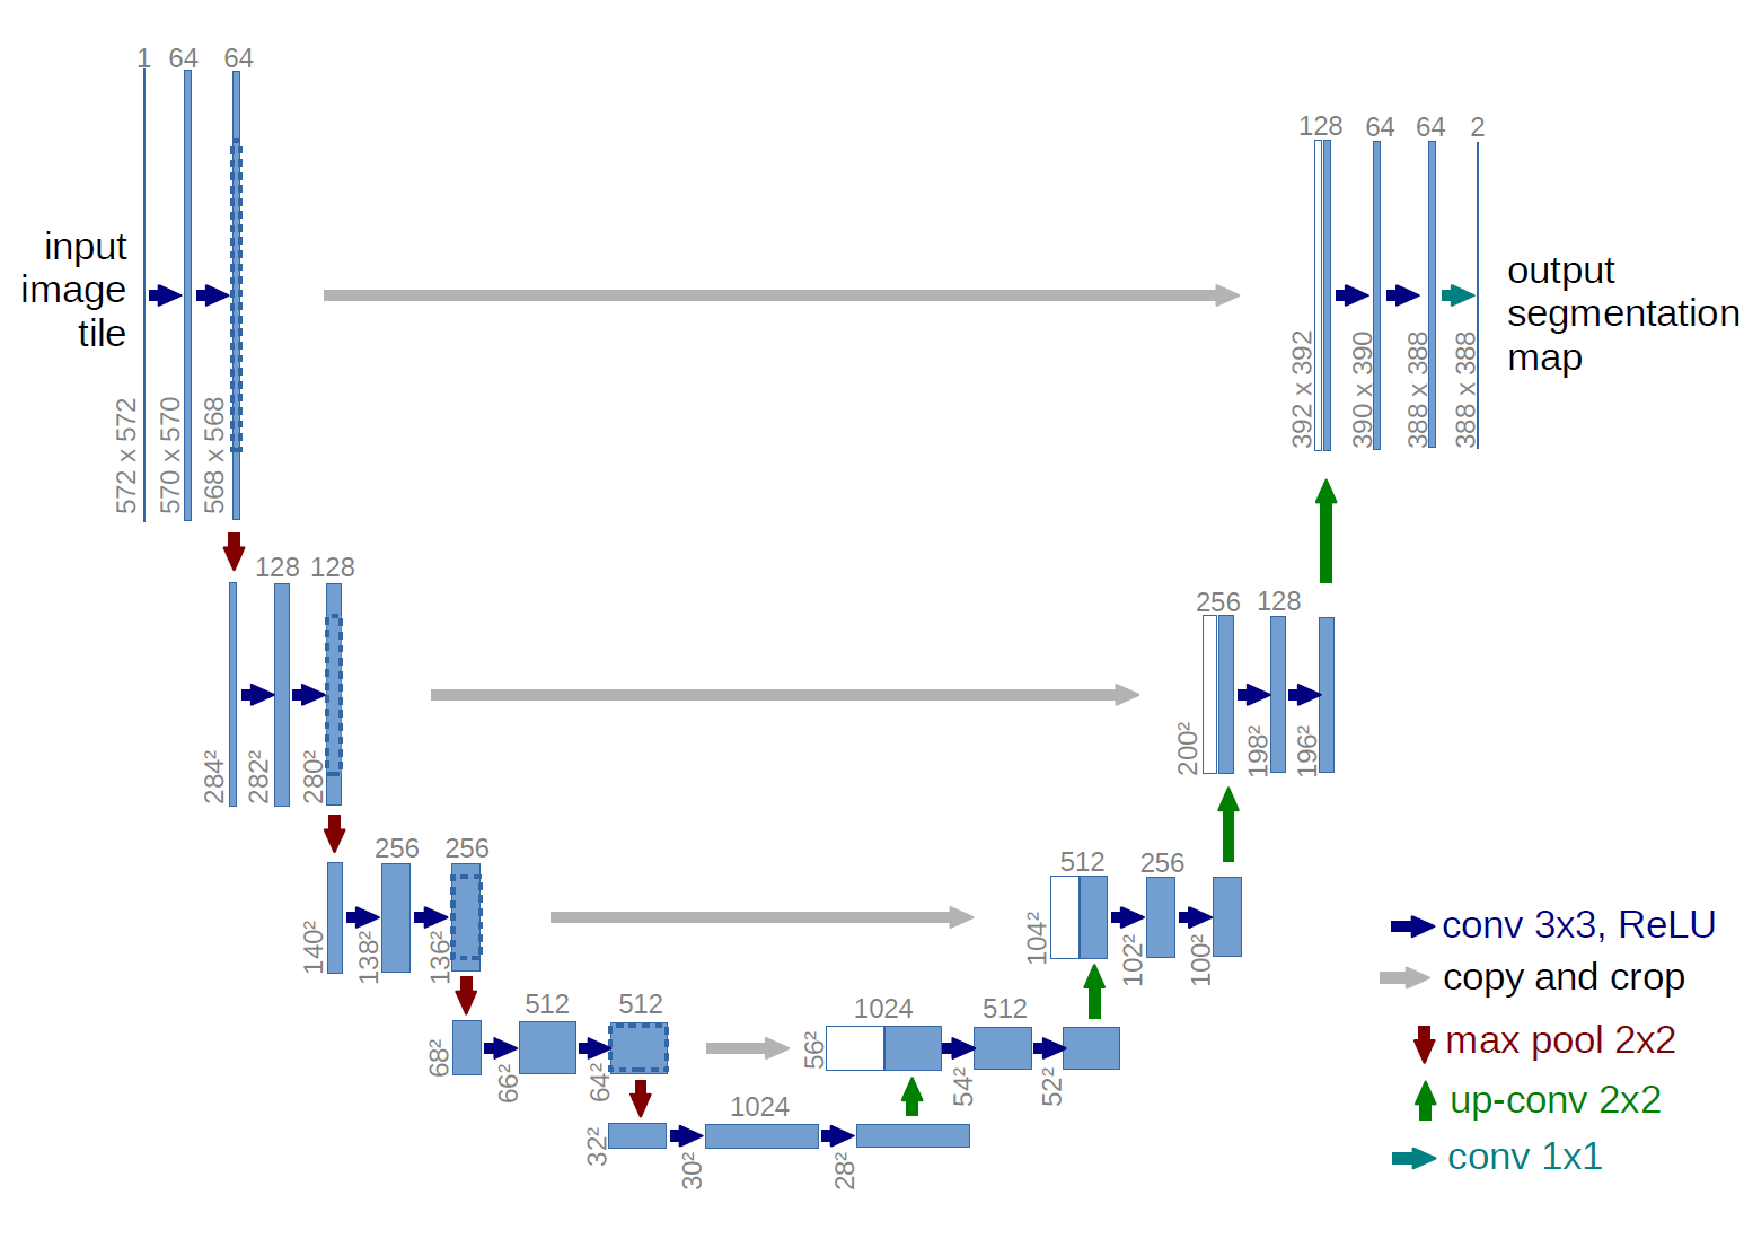
\includegraphics[width=\textwidth]{figures/130_methods/unet_nocaption.pdf}
}
\caption{\textbf{Unet architecture} \textit{(example for 32x32 pixels in the lowest resolution)}.
    Each blue box corresponds to a multi-channel feature map. The number of channels is denoted on top of the box. The x-y-size is provided at the lower left edge of the box. White
    boxes represent copied feature maps. The arrows denote the different operations.
    This figure is borrowed from \protect \citeA{unet}
} \label{fig:unet_architecture}
\end{figure}